\section{Pretrained models on the ladder}
\label{sec:s-models}
This section gives the protocol and the full results behind Section~4.4 and the model table of the main text.
The protocol was written before any full run was scored (\src{docs/PROTOCOL_model_fills.md}).

\paragraph{Models and weights.}
All weights are used as released; nothing is trained or tuned.
LaMa~\cite{lama2022} is run with two sets of weights: the model trained on CelebA-HQ at 256 pixels (\texttt{lama-celeba-hq/lama-fourier}, generator code of the authors' repository) and the large model trained on scenes (\texttt{big-lama}, Places).
Stable Diffusion 1.5 inpainting~\cite{rombach2022ldm} is run with an empty prompt, guidance scale 1, 20 steps at 512 pixels and one sample per region with a fixed seed.
The brain model is the first-ranked entry of the \ac{BraTS} 2024 inpainting challenge~\cite{brats2024winner}: a mean over 25 three-dimensional U-Net checkpoints, taken from the challenge container distributed by the \ac{BraTS} orchestrator~\cite{bratsorch2025}.
LaMa code is released under Apache 2.0, the Stable Diffusion weights under CreativeML OpenRAIL-M and the challenge weights under CC BY 4.0.

\paragraph{What a model sees and returns.}
In faces the model receives the whole aligned 128-pixel frame of the target, as standardized gray level mapped to $[0,1]$ by a fixed affine and repeated in three channels, with one window set to zero, together with the window mask.
The frame is brought to the model's resolution (256 pixels, 512 for the diffusion model) by an interpolation that reads visible pixels only: the bicubic interpolation of the frame with the window set to zero is divided by the same interpolation of the visibility mask.
No pixel that the model sees therefore depends on the hidden content or on a value we invented for it.
The output is averaged over channels, downsampled and mapped back; only the hidden window is kept.
In the brain the model receives the skull-stripped scan with one 16\,mm cube set to zero and the cube mask in the $240\times240\times155$ challenge grid.
The 1\,mm template grid is moved there by axis flips, zero padding and a 155-slice window, so neither the scan nor the fill is interpolated; interpolation would smooth the fill, which \ac{MSE} rewards.
We run the container's own preprocessing, forward pass and postprocessing in memory; on three cases the result equals the output of the official entry point up to $4\times10^{-7}$ of the cube maximum.
The returned cube is standardized with the target's own mean and standard deviation inside the brain mask.

\paragraph{Scoring and checks.}
A model fill is one more rung: it is scored by the same functions as the references on the same valid pixels, and the random-person scale uses the same 16 random people per target.
Before a model row was kept, the same call had to reproduce the stored rows of the references: every rung on the test targets, the dataset average and the second image on all 1{,}599 face targets (137{,}049 rows, largest difference $4\times10^{-15}$), and the dataset average in the brain.
The summary recomputes every reference value of the cross-dataset results from the stored rows and matches them exactly.
Intervals of the model rows are 95\% percentile intervals from 1{,}000 bootstrap draws over people (families in IMDb-WIKI), as in the cross-dataset results at 1/8 of the object.
\ac{LPIPS}, \ac{FID} and \ac{FWD} of the references exist only at the 16-pixel window in faces, so the face models were also run at that window and scored with the same functions; the stored \ac{LPIPS} of the dataset average and the stored \ac{FID} and \ac{FWD} of the random-person set are reproduced.
For every model we looked at sheets of evenly spaced targets, with the model fill next to the target and the references, before the full run was scored.

\paragraph{The pixels next to the mask decide the score.}
Two earlier ways of preparing the face input gave wrong positions, and we report them because the same mistakes are easy to make in any inpainting benchmark that resamples its images (Table~\ref{tab:s-input}).
In the first, the frame was upsampled before the window was masked, so the interpolation kernel carried the hidden values of the window's border into the visible pixels next to it; both LaMa models then scored closer to the target than with a clean input.
In the second, the window was filled with the mean of its surroundings before upsampling; this left a faint outline around the window, and the scene-trained model continued it as a dark frame inside the hole and scored almost as far as a random person in CelebA.
The input described above avoids both.
Two alternatives that also read visible pixels only, replicating pixels without interpolation and running the model at the 128-pixel frame without any resampling, were run on every eighth target and place each model within \mfSensSpread{} of the reported value.
A model's position on an error scale therefore depends on how the pixels next to the mask are prepared.

\begin{table}[htbp]
\centering
\caption{\textbf{The same model under five ways of preparing the masked face.}
\acs{MSE} on the random-person scale at 1/8 of the object, on every eighth target of each set (Targets).
Reported: interpolation from visible pixels only; replicated: pixel replication; native: model run at the frame resolution; outline and leak: the two discarded inputs, shown for the record; near: mean of the 16 nearest people on the same targets.
Compare each row from left to right: the three inputs that neither leak nor invent a value should agree, and the two discarded ones show how far the same model moves when the pixels next to the mask are wrong.}
\label{tab:s-input}
\small
\setlength{\tabcolsep}{4pt}
\begin{tabular}{@{}llrrrrrrr@{}}
\toprule
Set & Model & Targets & Reported & Replicated & Native & Outline & Leak & Near \\
\midrule
% Generated by paper/cvpr2027/make_model_fills.py from results/model_fills_v1/model_fills_input_sensitivity.json
n/a & not finished & & & & & & & \\
\bottomrule
\end{tabular}
\end{table}
% Source: results/model_fills_v1/model_fills_input_sensitivity.json; rows by make_model_fills.py.

\paragraph{Size of the hidden region.}
Table~\ref{tab:s-size} adds the two LaMa models to the size curve of the main text, on the same 100 evenly spaced targets per face set.
This analysis was added after the result at 1/8 was known and is exploratory.

\begin{table}[htbp]
\centering
\caption{\textbf{LaMa on the size curve in faces.}
\acs{MSE} on the random-person scale for hidden regions of 1/16, 1/8, 1/5 and 1/4 of the face width (5, 10, 16 and 20 pixels), 100 targets per set.
Read each column from top to bottom: a model above the row of the 16 nearest people is closer to the target than that retrieval baseline at this size.}
\label{tab:s-size}
\small
\begin{tabular}{@{}llrrrr@{}}
\toprule
Set & Fill & 1/16 & 1/8 & 1/5 & 1/4 \\
\midrule
% Generated by paper/cvpr2027/make_model_fills.py from results/model_fills_v1/model_fills_size_faces.json
CelebA & LaMa (CelebA-HQ) & 0.07 & 0.13 & 0.22 & 0.27 \\
CelebA & LaMa (Places) & 0.08 & 0.16 & 0.27 & 0.33 \\
CelebA & 16 nearest people & 0.11 & 0.19 & 0.26 & 0.27 \\
CelebA & Dataset average & 0.50 & 0.49 & 0.49 & 0.49 \\
CelebA & Same person & 0.64 & 0.63 & 0.63 & 0.63 \\
\midrule
IMDb-WIKI & LaMa (CelebA-HQ) & 0.09 & 0.15 & 0.22 & 0.27 \\
IMDb-WIKI & LaMa (Places) & 0.09 & 0.18 & 0.28 & 0.33 \\
IMDb-WIKI & 16 nearest people & 0.12 & 0.21 & 0.27 & 0.29 \\
IMDb-WIKI & Dataset average & 0.49 & 0.49 & 0.49 & 0.49 \\
IMDb-WIKI & Same person & 0.65 & 0.65 & 0.66 & 0.65 \\
\bottomrule
\end{tabular}
\end{table}
% Source: results/model_fills_v1/model_fills_size_faces.json; rows by make_model_fills.py.

\paragraph{Subsets.}
The two slow models ran on subsets fixed in advance by compute cost alone.
The diffusion model ran on every 16th person of each face set at 1/8 of the object (\mfSdCelebaN{} people in CelebA and \mfSdImdbN{} in IMDb-WIKI), and on the stored set-level regions at the 16-pixel window.
One brain cube costs 25 forward passes, so the brain ensemble ran on 8 of the 32 cubes (every fourth, both hemispheres) for targets taken in a fixed order: the 23 people with a second scan first, then the others in an order that spreads any prefix evenly over the cohort.
The run stopped on its time budget of six hours, not on a result, after \mfBratsQtimN{} people (all 23 with a second scan and 14 others).
For both models Table~\ref{tab:s-models} gives the reference values recomputed on the same targets.

\paragraph{Limits.}
Every model except the face-trained LaMa is used outside its training domain: a scene model and a text-to-image model on gray aligned faces, and a model trained to fill tumor regions on healthy young brains with small cubic masks.
CelebA-HQ is a subset of CelebA, so the face-trained LaMa may have seen CelebA people; IMDb-WIKI is its leakage-free set.
The array orientation of the challenge grid was set from the file convention of the challenge data, which we could not check against a challenge scan; on 18 test cubes other orientations gave slightly higher error (0.29 and 0.30 against 0.28 under \ac{MSE}).
The positions therefore describe what each metric rewards in these fills; they do not rank the models.

\begin{table}[htbp]
\centering
\caption{\textbf{Pretrained models: full results.}
Random-person scale at 1/8 of the object, with the 95\% bootstrap interval for \acs{MSE}; the four reference columns give \acs{MSE} on the same targets as the model (2nd: same person's second image; soft: softened; near: mean of the 16 nearest people; avg: dataset average).
\acs{LPIPS} (AlexNet), \acs{FID} and \acs{FWD} are from the 16-pixel window in faces; \acs{FID} and \acs{FWD} are divided by the distance of the random-person set (n/a: not computed).}
\label{tab:s-models}
\footnotesize
\setlength{\tabcolsep}{3.2pt}
\begin{tabular}{@{}llrlrrrrrrrrrrr@{}}
\toprule
 & & & & & & & & \multicolumn{4}{c}{\acs{MSE} of references} & & & \\
\cmidrule(lr){9-12}
Set & Model & Targets & \acs{MSE} & \acs{SSIM} & \acs{TM} & \acs{GDT} & \acs{lDDT} & 2nd & soft & near & avg & \acs{LPIPS} & \acs{FID} & \acs{FWD} \\
\midrule
% Generated by paper/cvpr2027/make_model_fills.py from results/model_fills_v1/model_fills_f8.json and results/model_fills_v1/model_fills_face_panel.json
QTIM & BraTS 2024 winner & 37 of 221 & 0.256 [0.238, 0.274] & 0.57 & 0.71 & 0.63 & 0.50 & 0.12 & 0.12 & 0.37 & 0.50 & n/a & n/a & n/a \\
CelebA & LaMa (CelebA-HQ) & 921 of 921 & 0.139 [0.136, 0.142] & 0.36 & 0.25 & 0.17 & 0.45 & 0.63 & 0.42 & 0.20 & 0.49 & n/a & n/a & n/a \\
CelebA & LaMa (Places) & 921 of 921 & 0.167 [0.163, 0.171] & 0.38 & 0.28 & 0.21 & 0.50 & 0.63 & 0.42 & 0.20 & 0.49 & n/a & n/a & n/a \\
IMDb-WIKI & LaMa (CelebA-HQ) & 678 of 678 & 0.151 [0.146, 0.156] & 0.40 & 0.27 & 0.19 & 0.50 & 0.68 & 0.44 & 0.21 & 0.49 & n/a & n/a & n/a \\
IMDb-WIKI & LaMa (Places) & 678 of 678 & 0.185 [0.178, 0.191] & 0.42 & 0.30 & 0.23 & 0.55 & 0.68 & 0.44 & 0.21 & 0.49 & n/a & n/a & n/a \\
\bottomrule
\end{tabular}
\end{table}
% Sources: results/model_fills_v1/model_fills_f8.json and model_fills_face_panel.json; rows by make_model_fills.py.

\begin{figure}[htbp]
\centering
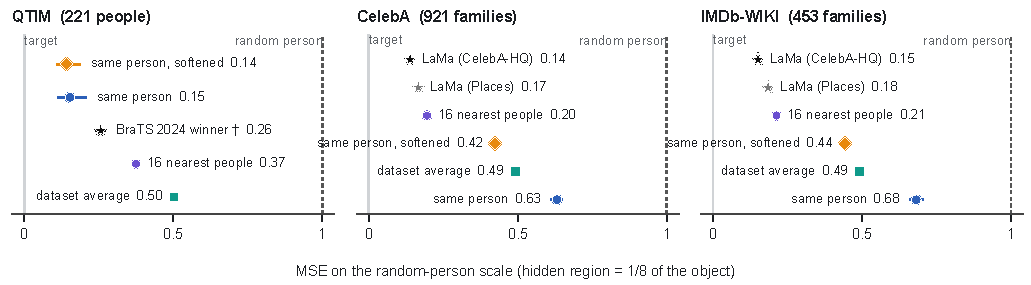
\includegraphics[width=\textwidth]{fig/model_fills_v1.pdf}
\caption{\textbf{Pretrained models and references under \acs{MSE}.}
Each panel is one image set and each row one fill: the references of the main text above the line, the models below it.
The horizontal position is the distance on the random-person scale with the hidden region at 1/8 of the object, with 95\% bootstrap intervals (often narrower than the marker); a dagger marks a model run on a subset of people.
Read each panel from left (the target) to right (a random person): in faces both LaMa models lie left of every reference, and in the brain the model lies between the same person's second scan and the mean of the 16 nearest people.}
\label{fig:s-models}
\end{figure}
